\documentclass[fontset=windows,12pt,a4paper,titlepage,UTF8]{ctexart}

\usepackage{amsmath}
\usepackage{tabularx}
\usepackage{booktabs}
\usepackage{hyperref}
\usepackage{subcaption}
\usepackage{graphicx}
\usepackage{svg}
\usepackage{multicol}
\usepackage{multirow}
\usepackage{makecell}
\usepackage{siunitx}

% \setCJKmainfont{Noto Serif CJK SC}
% \setCJKsansfont{Noto Sans CJK SC}
% \setCJKmonofont{Noto Sans Mono CJK SC}
% \setmainfont{Noto Serif}
% \setsansfont{Noto Sans}
% \setmonofont{Noto Sans Mono}

\hypersetup{colorlinks,allcolors=blue}

\sisetup{detect-all}

\author{石成玉}
\date{\today}
\title{基于超声波振动的肥箱抗粘减阻装置设计}

\begin{document}

\maketitle

\begin{abstract}

  土壤肥力直接影响果树的生长、产量和品质及果园的可持续健康发展。土壤有机质是衡量土壤肥力的重要标准,决定了土壤肥力的物质基础,也是保障果树高产、优质的重要条件。果园施用有机肥可以有效增加土壤有机质含量,改善土壤结构及理化性状,是果园产业实现高质量高效率发展的关键之一。

  目前,果园有机肥施肥机已进行了大量研究,但由于高湿有机肥容易与肥箱底板内部粘附,导致施肥机排肥装置阻力增大,严重时会引起肥料堵塞现象,极大的影响了作业质量与效率,因此减小有机肥施肥机排肥作业阻力已成为亟待解决的问题。针对以上情况,本文设计了一种基于超声波震动的肥箱抗粘减阻装置。本文通过对比有无震动时有机肥料与肥箱底板的摩擦因数,确定了超声波震动技术对于抗粘减阻有显著的效果。随后,本文通过多普勒震动扫描仪确定超声波在钢板上的衰减规律,作为之后建立有限元分析的模型的准确性的验证。进一步,本文在COMSOL软件中建立了超声波换能器与钢板的有限元模型,分析和确定了超声波换能器的最佳型号选择和最佳布置方式。

\end{abstract}

\tableofcontents

\newpage

\section{研究背景}

中国水果产业品类多、总量大,果园总面积和水果总产量年稳居世界首位。近年来,中国水果产业快速发展,呈现面积稳中有增、产量稳步提高、区域优势品种愈加突出、增收作用日益提升的良好局面,已成为农业农村经济发展的重要支柱产业。我国果品的生产总量、栽培面积及资源种类均居于世界首位。我国虽然是世界水果生产大国之一,但并不是世界水果生产强国,我国水果产业没有充分发挥我国所有的自然资源优势。其中,我国水果出口贸易发展中存在的国际影响力弱,水果竞争力弱等问题,最根本的原因是我国果品品质差、劣质品种多。因此,要全面提高我国水果产业在国际市场上的竞争力,改变我国水果产业大而不强的现状,充分利用我国的自然资源,必须从根本上改善我国水果品质差的问题,生产高品质水果以改变产业大而不强的现状。

水果产业发展不仅需要产量大,还需要品质高。其中,土壤有机物含量是影响水果品质的重要因素。富含有机物的土壤不仅营养充足,相对于有机物含量较少的土壤还能支撑水分净化、保持和供应。好的果园土壤的有机质含量应在3.0\%以上,而中国果园的土壤有机质含量普遍在1.0\%左右,属于偏低水平,与国外有较大差距。因此,造成中国水果产业国际竞争力差的主要原因就是土壤有机质含量过低。

要提高土壤有机质含量的方法就是施用有机肥。而人工施有机肥存在很多问题。首先,人工劳动成本高、劳动强度高。其次,人工施肥不够精准,会导致施肥不均匀和浪费。机械施肥虽然能解决人工施肥的一些问题,但是同时也引入了新的问题。施肥机器在施有机肥时普遍存在有机肥粘附,甚至堵塞肥箱的问题。随着科学技术的进步,农业领域的减粘脱附技术已有一些进步,比如改变表面形貌减粘脱附技术、机械减粘脱附技术、加热减粘脱附技术等,都有其局限性。

震动减租技术具有效果好、功耗低的优点。在部分领域已有应用,在金属加工领域中就有使用超声波震动技术降低加工金属时切削的阻力,可以显著降低切削的阻力。可以将该技术带到农业机械领域来。

综上所述,本研究先确定超声波震动减阻在有机肥施肥机械上的减阻效果。再通过有限元分析技术,确定最佳的超声波震动的频率和功率以及布置方式。

\section{超声波震动对有机肥与钢板摩擦角影响}

本章节通过试验的方法,研究在超声波震动的影响下,有机肥与钢板的摩擦角的变化情况。并设计试验确定有机肥含水量、震动功率、震动频率对摩擦角的影响程度。

\subsection{摩擦角试验}

\subsubsection{试验材料}

\paragraph{有机肥颗粒}

试验采用的是陕西睿浩生物有限公司生产的商用有机肥原始含水率为37.43\%,通过自然风干法和添加纯净水方法配置6个含水率梯度10\%、20\%、30\%、40\%、50\%、60\%。6种不同湿度有机肥如图\ref{pic:有机肥含水量梯度}所示。

\begin{figure}[h]
  \centering
  \begin{subfigure}[h]{0.3\textwidth}
    \centering
    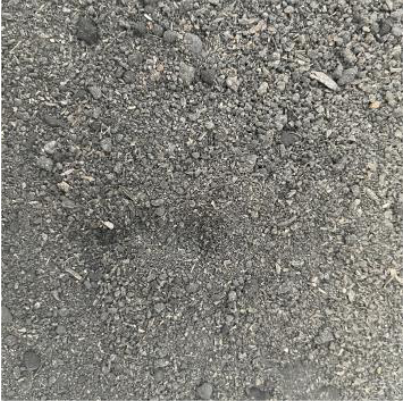
\includegraphics{assets/organic_fertilizer_moisture_10.png}
    \caption{含水量10\%}
    \label{pic:有机肥含水量10}
  \end{subfigure}
  \hfill
  \begin{subfigure}[h]{0.3\textwidth}
    \centering
    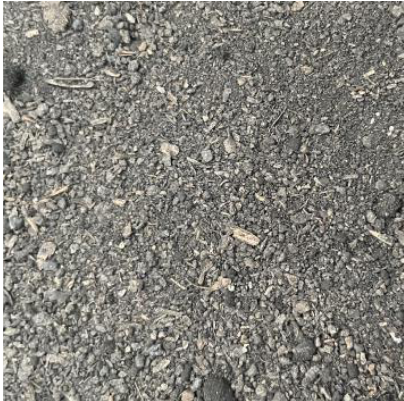
\includegraphics{assets/organic_fertilizer_moisture_20.png}
    \caption{含水量20\%}
    \label{pic:有机肥含水量20}
  \end{subfigure}
  \hfill
  \begin{subfigure}[h]{0.3\textwidth}
    \centering
    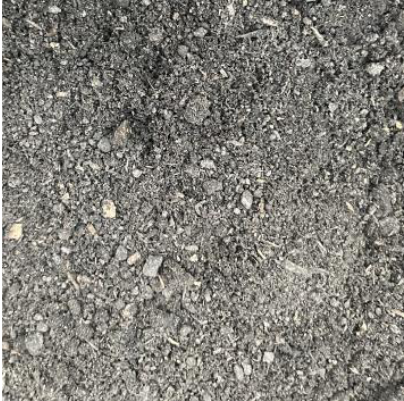
\includegraphics{assets/organic_fertilizer_moisture_30.png}
    \caption{含水量30\%}
    \label{pic:有机肥含水量30}
  \end{subfigure}

  \vspace{1em}

  \begin{subfigure}[h]{0.3\textwidth}
    \centering
    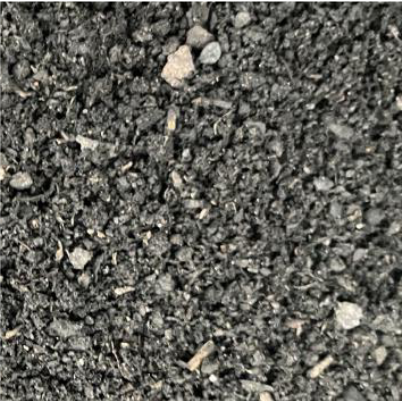
\includegraphics{assets/organic_fertilizer_moisture_40.png}
    \caption{含水量40\%}
    \label{pic:有机肥含水量40}
  \end{subfigure}
  \hfill
  \begin{subfigure}[h]{0.3\textwidth}
    \centering
    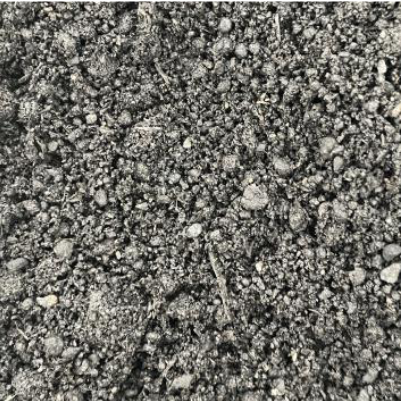
\includegraphics{assets/organic_fertilizer_moisture_50.png}
    \caption{含水量50\%}
    \label{pic:有机肥含水量50}
  \end{subfigure}
  \hfill
  \begin{subfigure}[h]{0.3\textwidth}
    \centering
    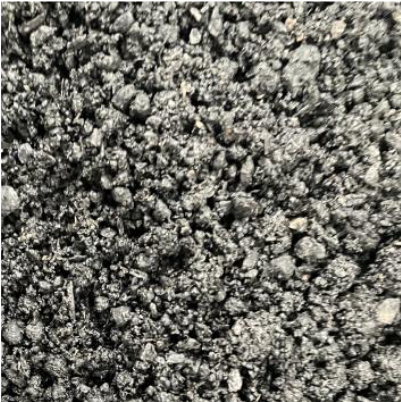
\includegraphics{assets/organic_fertilizer_moisture_60.png}
    \caption{含水量60\%}
    \label{pic:有机肥含水量60}
  \end{subfigure}

  \caption{不同含水量的有机肥}
  \label{pic:有机肥含水量梯度}
\end{figure}

\paragraph{超声波换能器}

超声波换能器主要工作部件是压电材料,它可以将交流电转化为机械震动,机械震动的频率与交流电的频率成正比,机械震动的幅度与电压成正比。本研究所使用的三种不同频率的夹心压电超声换能器如图\ref{pic:超声波换能器}所示,该超声换能器型号为HS-8SH-38。

\begin{figure}[h]
  \centering
  \begin{subfigure}{0.3\textwidth}
    \centering
    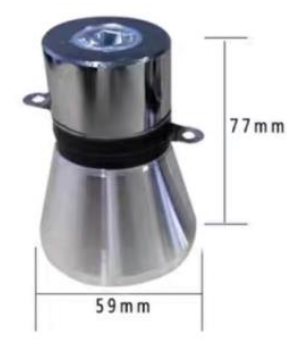
\includegraphics{assets/Ultrasonic_transducer_25kHz.png}
    \caption{25kHz}
    \label{pic:换能器25}
  \end{subfigure}
  \hfill
  \begin{subfigure}{0.3\textwidth}
    \centering
    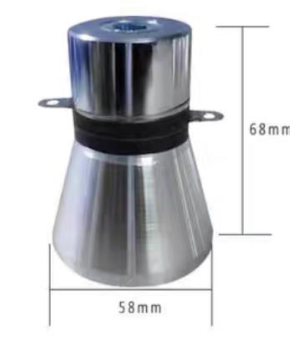
\includegraphics{assets/Ultrasonic_transducer_28kHz.png}
    \caption{28kHz}
    \label{pic:换能器28}
  \end{subfigure}
  \hfill
  \begin{subfigure}{0.3\textwidth}
    \centering
    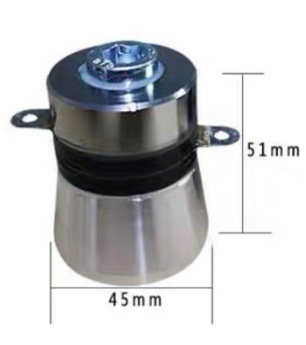
\includegraphics{assets/Ultrasonic_transducer_40kHz.png}
    \caption{40kHz}
    \label{pic:换能器40}
  \end{subfigure}
  \caption{超声波换能器}
  \label{pic:超声波换能器}
\end{figure}

\paragraph{钢板}

实验所用钢板材料为Q235钢,与肥箱底部钢板材料一致。钢板尺寸为$600 \mathrm{mm} \times 600\mathrm{mm}$。

\subsubsection{实验方案}

实验通过测试加超声波振动和不加超声波振动两种情况下的有机肥与钢板的静摩擦角来检测超声波的减阻效果。实验装置如图\ref{pic:静摩擦角检测试验装置示意图}所示,有机肥放在钢板上,在钢板的底部布置超声波换能器,同时在钢板上安装角度仪。实验时,缓慢地逆时针转动钢板,记录有机肥开始动的瞬间的角度。

\begin{figure}[h]
  \centering
  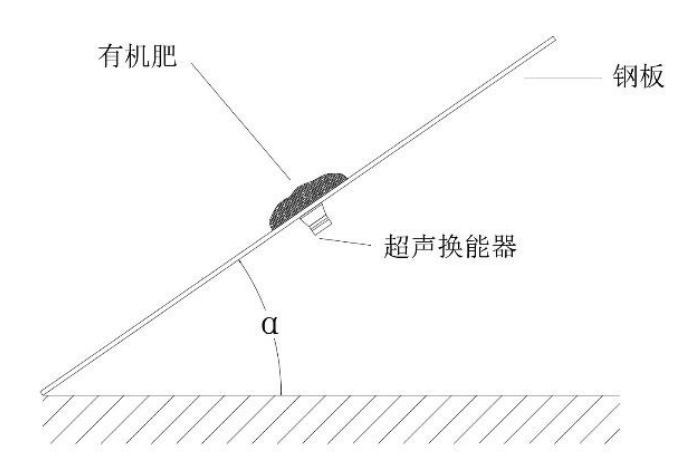
\includegraphics[width=0.4\textwidth]{assets/experiment.png}
  \caption{静摩擦角检测试验装置示意图}
  \label{pic:静摩擦角检测试验装置示意图}
\end{figure}

为了对比减阻效果的强弱,在此定义减阻率$\beta$,即施加超声波振动后降低的摩擦角相对无超声波振动的摩擦角的比例,如公式\eqref{eq:减阻率}所示:

\begin{equation}
  \beta = \frac{\tan \alpha_0 - \tan \alpha_1}{\tan \alpha_0} \label{eq:减阻率}
\end{equation}

\subsubsection{试验方案}

预实验后筛选出3个影响减阻率的因素:

\begin{enumerate}
  \item\textbf{超声波振动频率}:目前超声振动换能器主要有25kHz、28kHz和40kHz,因此本研究控制超声振动频率为25kHz、28kHz和40kHz,共3个频率水平
  \item\textbf{超声波换能器功率}:考虑到换能器最大输入功率为60W,因此本研究控制超声振动功率为10-60W,期间每10W为1个梯度,共6个功率水平
    % \item\textbf{钢板厚度}:由于肥箱底部钢板厚度一般为2mm左右,因此本研究控制Q235钢板厚度为15mm,每1mm为1个梯度,共5个水平。
  \item\textbf{有机肥含水率}:由于有机肥含水率范围较广,容易吸收空气中水分,因此本研究控制有机肥含水率为10\%-60\%,每10\%为一个梯度,共6个水平。
\end{enumerate}

针对3个影响因素设计正交试验,正交试验具体方案如表\ref{tb:正交试验方案}所示,正交试验的结果如图\ref{pic:正交试验结果}所示。

\begin{table}[h]
  \centering
  \caption{正交试验方案}
  \label{tb:正交试验方案}
  \begin{tabular}{S c c c S S}
    \toprule
    {\textbf{试验序号}} & {\textbf{功率(\unit{\watt})}} & {\textbf{频率(\unit{\kilo\hertz})}} & {\textbf{有机肥含水率}} & {\textbf{摩擦角}(\unit{\degree})} & {\textbf{减阻率}} \\
    \midrule
    1 & 35 & 40 & 60\% & 34.93 & 30.86\% \\
    2 & 60 & 40 & 35\% & 30.39 & 18.53\% \\
    3 & 35 & 28 & 35\% & 28.80 & 23.63\% \\
    4 & 60 & 25 & 35\% & 28.89 & 23.35\% \\
    5 & 10 & 28 & 60\% & 25.9 & 51.93\% \\
    6 & 60 & 28 & 10\% & 14.71 & 46.83\% \\
    7 & 35 & 25 & 10\% & 24.1 & 9.42\% \\
    8 & 35 & 28 & 35\% & 28.80 & 23.63\% \\
    9 & 10 & 40 & 35\% & 34.36 & 5.03\% \\
    10 & 10 & 25 & 35\% & 32.11 & 12.83\% \\
    11 & 60 & 28 & 60\% & 19.8 & 64.36\% \\
    12 & 35 & 25 & 60\% & 29.7 & 43.53\% \\
    13 & 35 & 40 & 10\% & 24.84 & 6.25\% \\
    14 & 10 & 28 & 10\% & 22.05 & 17.97\% \\
    15 & 35 & 28 & 35\% & 28.80 & 23.63\% \\
    \bottomrule
  \end{tabular}
\end{table}

\begin{figure}[h]
  \centering
  \begin{subfigure}{0.3\textwidth}
    \centering
    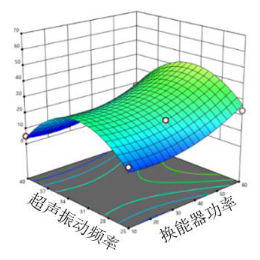
\includegraphics[width=\textwidth]{assets/frequency_power.png}
  \end{subfigure}
  \hfill
  \begin{subfigure}{0.3\textwidth}
    \centering
    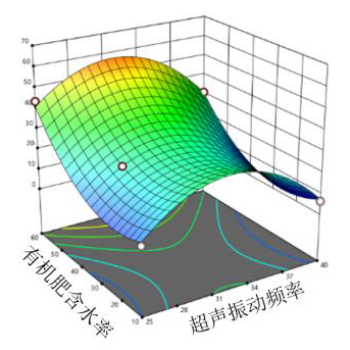
\includegraphics[width=\textwidth]{assets/moisture_frequency.png}
  \end{subfigure}
  \hfill
  \begin{subfigure}{0.3\textwidth}
    \centering
    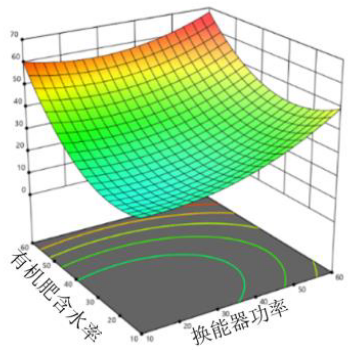
\includegraphics[width=\textwidth]{assets/moisture_power.png}
  \end{subfigure}
  \caption{正交试验结果}
  \label{pic:正交试验结果}
\end{figure}

正交试验的结果表明超声振动对有机肥的摩擦角影响显著,其中在28kHz的超声振动频率下,对有机肥的摩擦角影响最显著;有机肥的含水率越高,超声减阻效果越好,有机肥的含水率达到60\%时,超声振动减阻率可高达57.26\%;超声振动功率越大减阻效果越好,功率大于40W时,减阻效果趋于稳定。

\section{单换能器振幅分布试验与仿真模型建立}

为了研究最佳的超声波换能器布置方式,需要对其建模进行有限元仿真分析。因此,首先要通过实际试验寻找超声波振动在钢板上的衰减规律,为后续的有限元仿真模型做标定,确保模型的可用性。

\subsection{单换能器振幅分布试验}

\subsubsection{试验材料与方法}

本试验采用PSV-400-M2多普勒激光测振仪测量单换能器激励下的超声振动振幅分布,可以在不接触被测量物体表面的情况下较远距离对物体表面的振动速度和位移进行测量。本次试验所搭建的测试平台如图\ref{pic:超声振动振幅分布测试平台}所示。其中,钢板尺寸为600mm$\times$600mm$\times$2mm,并且对钢板进行四边固定约束,以模拟其安装在施肥机上的真实情况。

\begin{figure}[h]
  \centering
  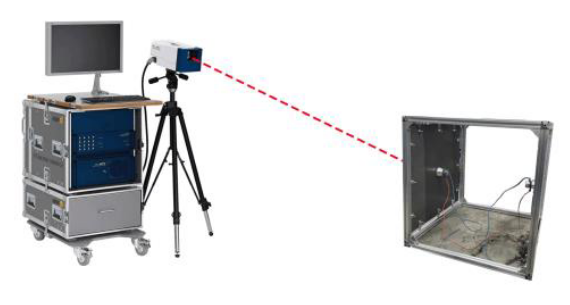
\includegraphics[width=0.8\textwidth]{assets/experiment_platform.png}
  \caption{超声振动振幅分布测试平台}
  \label{pic:超声振动振幅分布测试平台}
\end{figure}

试验选择了25kHz和28kHz两种超声波换能器分别进行测试。

\subsubsection{试验结果}

试验结果如图\ref{pic:不同频率的超声振动振幅分布}所示。

\begin{figure}[h]
  \centering
  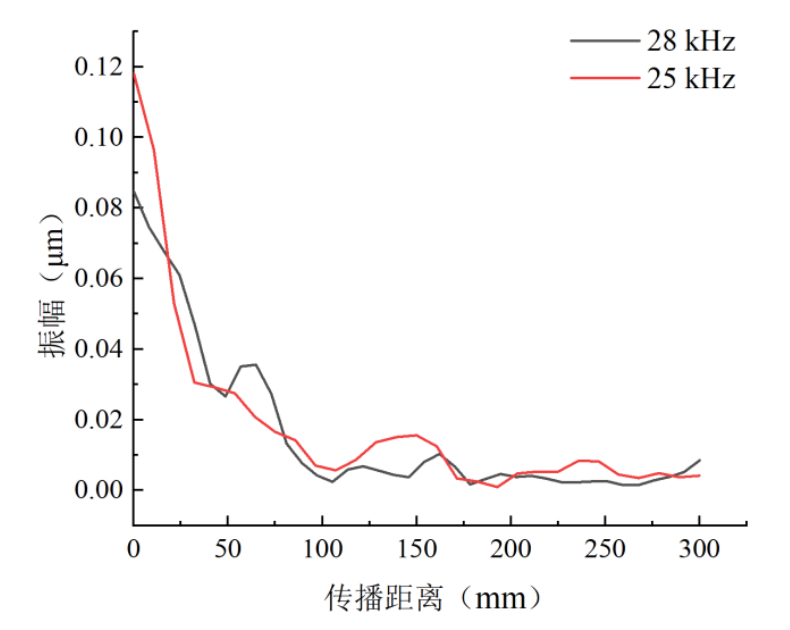
\includegraphics[width=0.6\textwidth]{assets/wave_spread.png}
  \caption{不同频率的超声振动振幅分布}
  \label{pic:不同频率的超声振动振幅分布}
\end{figure}

由图\ref{pic:不同频率的超声振动振幅分布}可知,在换能器中心位置处的振幅较大,超声振动对有机肥摩擦系数的影响效果最好,随着传播距离增加,有机肥摩擦系数逐渐增大,超声减阻效果降低。

由于超声振动在0mm--100mm的传播距离内衰减较快,因此有机肥摩擦角上升迅速。随着传播距离的增加,超声振动的衰减速度变慢,振幅减小幅度减小,有机肥摩擦系数的变化也减小。当传播距离大于260mm时,超声振幅减小到一定程度后,振幅对有机肥摩擦角的影响明显减小,无法改变有机肥颗粒与Q235钢板的摩擦特性。有机肥颗粒与Q235钢板的有效接触面积增大,减阻效果逐渐消失。

\subsection{有限元模型建立}

\subsubsection{材料参数}

使用COMSOL软件建立超声波换能器和钢板的有限元模型。其中所使用到的材料的各项参数如表\ref{tb:材料参数}所示。

\begin{table}[!h]
  \centering
  \caption{材料参数}
  \label{tb:材料参数}
  \begin{tabularx}{\textwidth}{
      >{\centering\arraybackslash}X
      >{\centering\arraybackslash}X
      >{\centering\arraybackslash}X
      >{\centering\arraybackslash}X
    }
    \toprule
    {\textbf{组成部分}} & {\textbf{材料类型}} & {\textbf{材料参数}} & {\textbf{参数值}} \\
    \midrule
    \multirow{5}{*}{后端盖} & \multirow{5}{*}{铝} & 密度(\unit{kg/m^3}) & 2770 \\
    & & 弹性模量(\unit{Pa}) & \num{7.1e10} \\
    & & 泊松比 & 0.33 \\
    & & 体积模量(\unit{Pa}) & \num{6.96e10} \\
    & & 剪切模量(\unit{Pa}) & \num{2.67e10} \\
    \midrule
    \multirow{5}{*}{前端盖} & \multirow{5}{*}{钢} & 密度(\unit{kg/m^3}) & 7750 \\
    & & 弹性模量(\unit{Pa}) & \num{1.93e11} \\
    & & 泊松比 & 0.33 \\
    & & 体积模量(\unit{Pa}) & \num{1.69e11} \\
    & & 剪切模量(\unit{Pa}) & \num{7.37e10} \\
    \midrule
    \multirow{5}{*}{钢板} & \multirow{5}{*}{Q235} & 密度(\unit{kg/m^3}) & 7850 \\
    & & 弹性模量(\unit{Pa}) & \num{2.05e11} \\
    & & 泊松比 & 0.29 \\
    \midrule
    压电陶瓷 & PZT4 & 密度(\unit{kg/m^3}) & 7500 \\
    \bottomrule
  \end{tabularx}
\end{table}

\subsubsection{压电材料域-超声波换能器的有限元模型}

\paragraph{支配方程}

超声波换能器的结构如图\ref{pic:超声波换能器结构}所示,超声波换能器的有限元模型如图\ref{pic:超声波换能器有限元模型}所示。由于超声波换能器不是主要研究对象,因此在有限元模型中对其做了合理的简化处理,即其前后端盖直接连接为一体。

\begin{figure}[h]
  \centering
  \begin{subfigure}{0.4\textwidth}
    \centering
    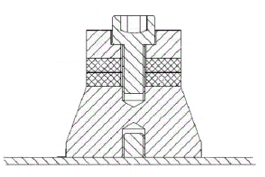
\includegraphics[width=0.6\textwidth]{assets/ultrasonic_transducer_structure.png}
    \caption{超声波换能器结构}
    \label{pic:超声波换能器结构}
  \end{subfigure}
  \hfil
  \begin{subfigure}{0.4\textwidth}
    \centering
    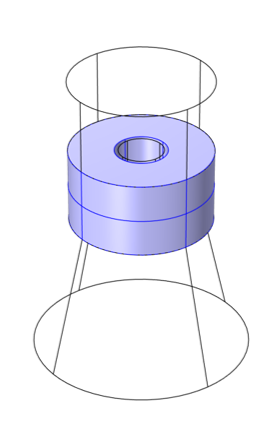
\includegraphics[width=0.6\textwidth]{assets/ultrasonic_transducer_model.png}
    \caption{超声波换能器有限元模型}
    \label{pic:超声波换能器有限元模型}
  \end{subfigure}
  \caption{超声波换能器}
\end{figure}

换能器核心部件为中间的压电材料,其支配方程如式所示:

\begin{equation}
  \nabla \cdot \mathbf{D} = \rho_v, \quad E = - \nabla V
  \label{eq:压电材料支配方程}
\end{equation}

\begin{table}[!h]
  \centering
  \begin{tabular}{l l}
    $\mathbf{D}$ & \text{电场位移} \\
    $\nabla$ & \text{散度运算符} \\
    $\rho_v$ & \text{自由电荷体密度} \\
    $V$ & \text{电势} \\
    $\nabla V$ & \text{梯度运算符} \\
    $E$ & \text{电场强度}
  \end{tabular}
\end{table}

\paragraph{边界条件}

超声波换能器的边界条件即压电材料的边界条件,其边界条件如下:

\begin{enumerate}
  \item 在两块压电材料的接触面如图\ref{pic:边界条件:交流电}所示,施加电压为133V频率为28kHz的交流电,即
    \begin{equation}
      V=133 \times \sin {(2 \times 28000 \times \pi \cdot t)}
      \label{eq:压电材料电压}
    \end{equation}
  \item 在两块压电材料各自的非接触面如图\ref{pic:边界条件:接地}所示,设置接地,即
    \begin{equation}
      V=0
      \label{eq:接地}
    \end{equation}
\end{enumerate}

\begin{figure}[h]
  \centering
  \begin{subfigure}{0.4\textwidth}
    \centering
    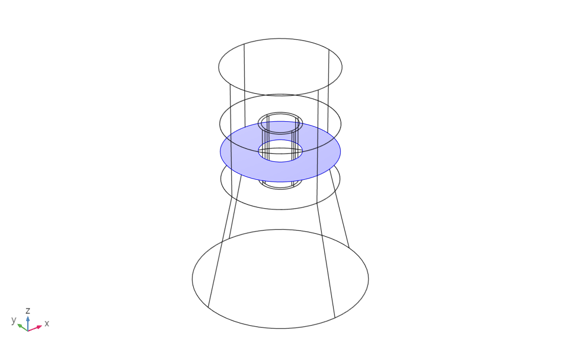
\includegraphics[width=\textwidth]{assets/ultrasonic_transducer_boundry_condition_v1.png}
    \caption{边界条件:交流电}
    \label{pic:边界条件:交流电}
  \end{subfigure}
  \hfill
  \begin{subfigure}{0.4\textwidth}
    \centering
    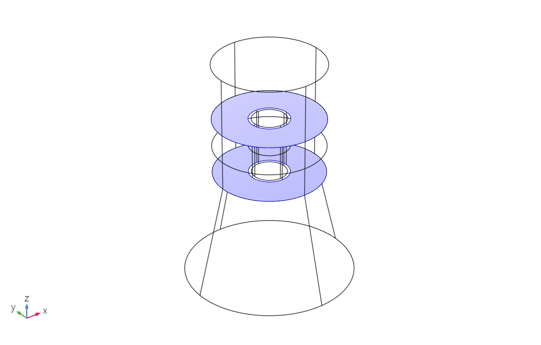
\includegraphics[width=\textwidth]{assets/ultrasonic_transducer_boundry_condition_v0.png}
    \caption{边界条件:接地}
    \label{pic:边界条件:接地}
  \end{subfigure}
  \caption{超声波换能器边界条件}
\end{figure}

\subsubsection{固体力学域-钢板和超声波换能器}

超声波换能器的外壳和钢板都处在固体力学域中。

\paragraph{整体模型}

所建立的模型如图\ref{pic:固体力学域模型}所示。其中,钢板的尺寸与实际试验所用的钢板尺寸一致,均为$600 \mathrm{mm} \times 600 \mathrm{mm} \times 2 \mathrm{mm}$。

\begin{figure}[h]
  \centering
  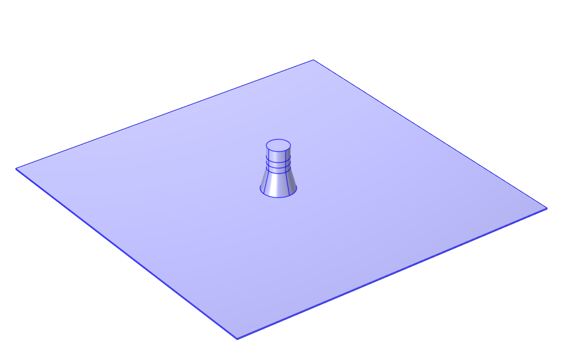
\includegraphics[width=0.6\textwidth]{assets/ultrasonic_transducer_plate_model.png}
  \caption{固体力学域模型}
  \label{pic:固体力学域模型}
\end{figure}

\paragraph{支配方程}

支配方程如式\eqref{eq:固体力学支配方程}所示。

\begin{equation}
  \rho \frac{\partial^2 \mathbf{u}}{\partial t^2} = \nabla (\mathbf{F}S)^2 + F_v, \quad F_v = 1 + \nabla \mathbf{u}
  \label{eq:固体力学支配方程}
\end{equation}

\paragraph{边界条件}

钢板的边界条件为四个侧边施加固定约束,即:

\begin{equation}
  \mathbf{u} = 0
  \label{eq:钢板边界条件}
\end{equation}

\subsection{有限元模型的验证}

为了确保所建立的有限元模型可用,需要将同等条件的仿真结果与实际试验进行对比。该模型的仿真结果如图\ref{pic:仿真结果}所示。

\begin{figure}[h]
  \centering
  \begin{subfigure}{0.45\textwidth}
    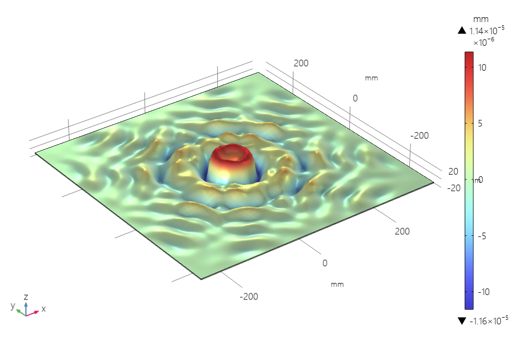
\includegraphics[width=\textwidth]{assets/result_600x600_proper_focus.png}
  \end{subfigure}
  \hfill
  \begin{subfigure}{0.45\textwidth}
    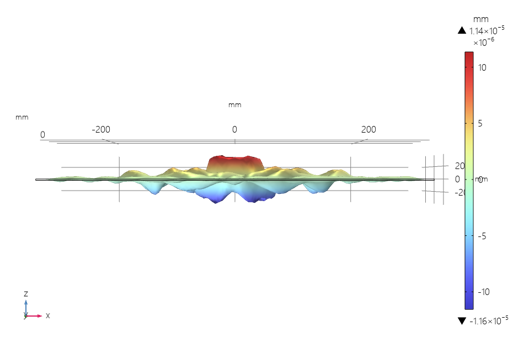
\includegraphics[width=\textwidth]{assets/result_600x600_side_focus.png}
  \end{subfigure}
  \caption{仿真结果}
  \label{pic:仿真结果}
\end{figure}

仿真结果与实际试验结果(图\ref{pic:不同频率的超声振动振幅分布})基本吻合,可认为该有限元模型可用。

\section{超声波换能器配置方案}

通过先前建立的有限元模型对超声波换能器安装在肥箱底部钢板的情况进行仿真,以确定有效振动的覆盖情况以及确定使用多个超声波换能器的情况下的最佳布置方案。

\subsection{单换能器仿真}

采用与实际肥箱底板规格相同的$1600 \mathrm{mm} \times 700 \mathrm{mm} \times 2 \mathrm{mm}$钢板,将超声波换能器安装在钢板中心,仿真结果如图\ref{pic:单换能器仿真结果}所示。

\begin{figure}[h]
  \centering
  \begin{subfigure}{0.45\textwidth}
    \centering
    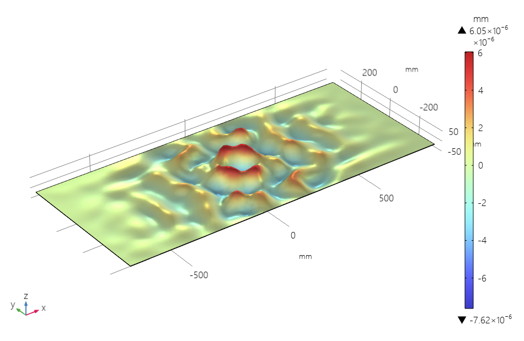
\includegraphics[width=\textwidth]{assets/result_1600x700_proper_focus.png}
  \end{subfigure}
  \hfill
  \begin{subfigure}{0.45\textwidth}
    \centering
    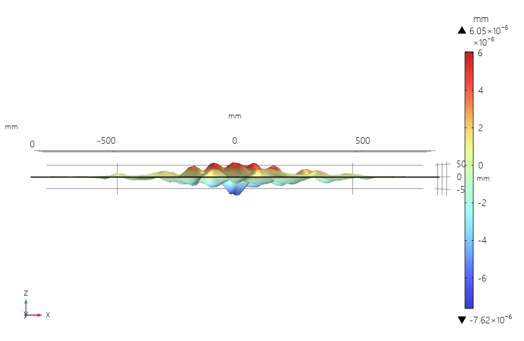
\includegraphics[width=\textwidth]{assets/result_1600x700_side_focus.png}
  \end{subfigure}
  \caption{单换能器仿真结果}
  \label{pic:单换能器仿真结果}
\end{figure}

从结果中可以看出,单个换能器的有效振动覆盖范围大约为直径700mm的圆。

\subsection{多换能器布置方案}

根据仿真结果提出两种多换能器布置方案,如图\ref{pic:多换能器布置方案}所示。

\begin{figure}[h]
  \centering
  \begin{subfigure}{0.4\textwidth}
    \centering
    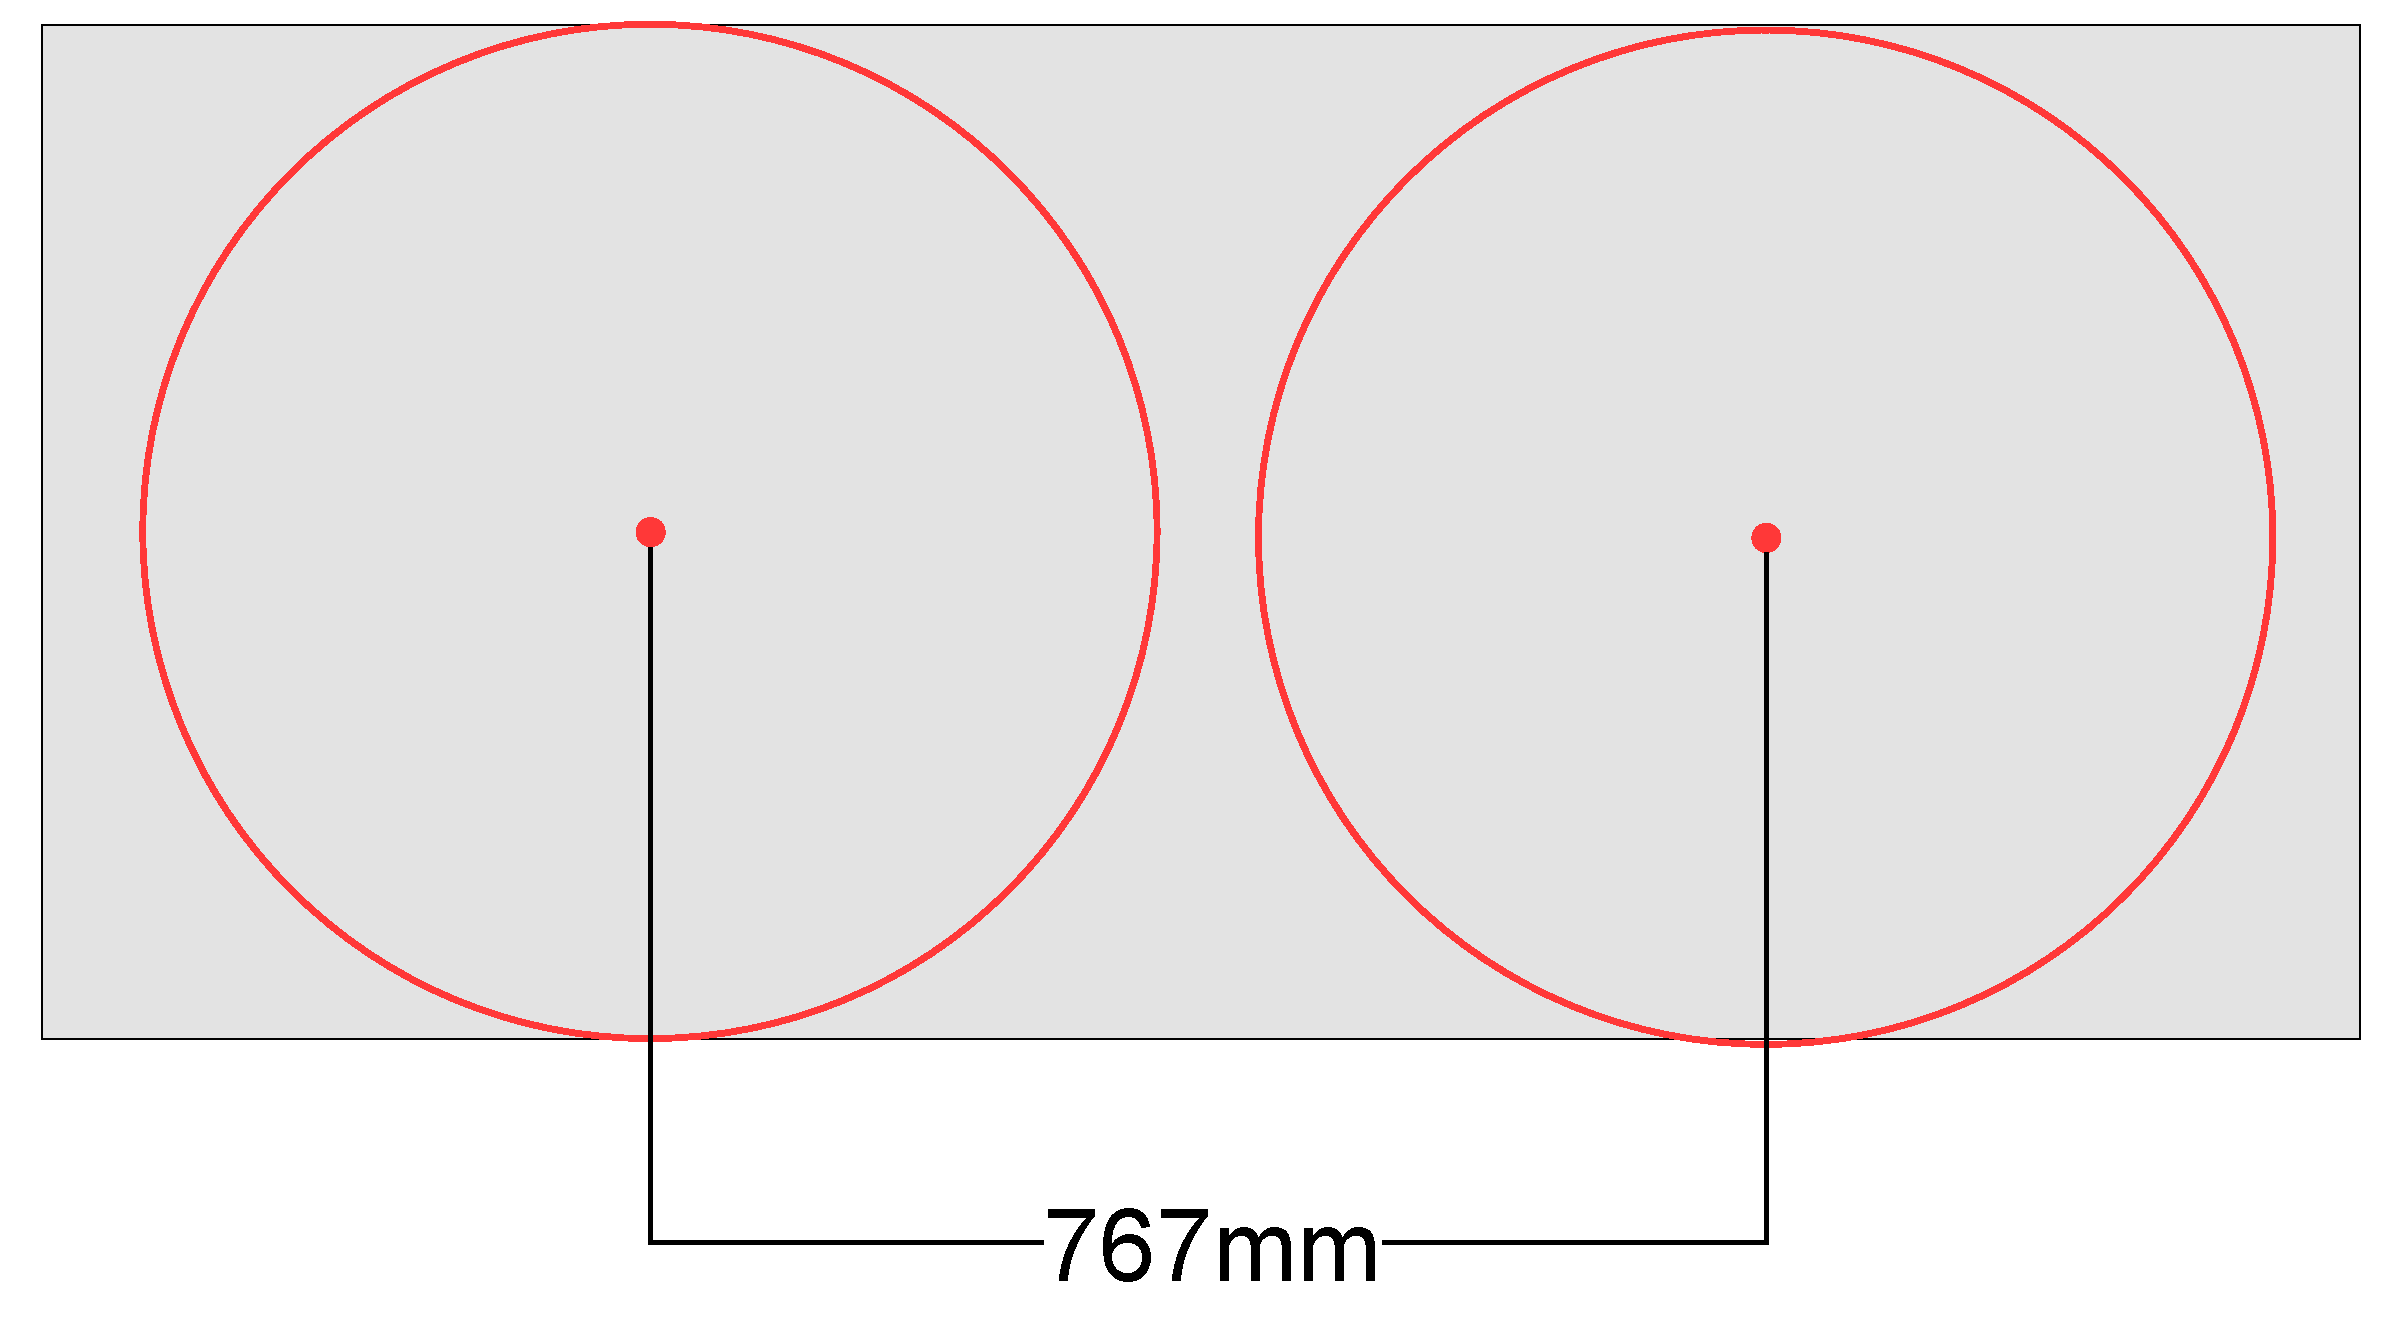
\includegraphics[height=5em]{assets/2transducer.pdf}
    \caption{2个换能器布置方案}
    \label{pic:2个换能器布置方案}
  \end{subfigure}
  \hfill
  \begin{subfigure}{0.5\textwidth}
    \centering
    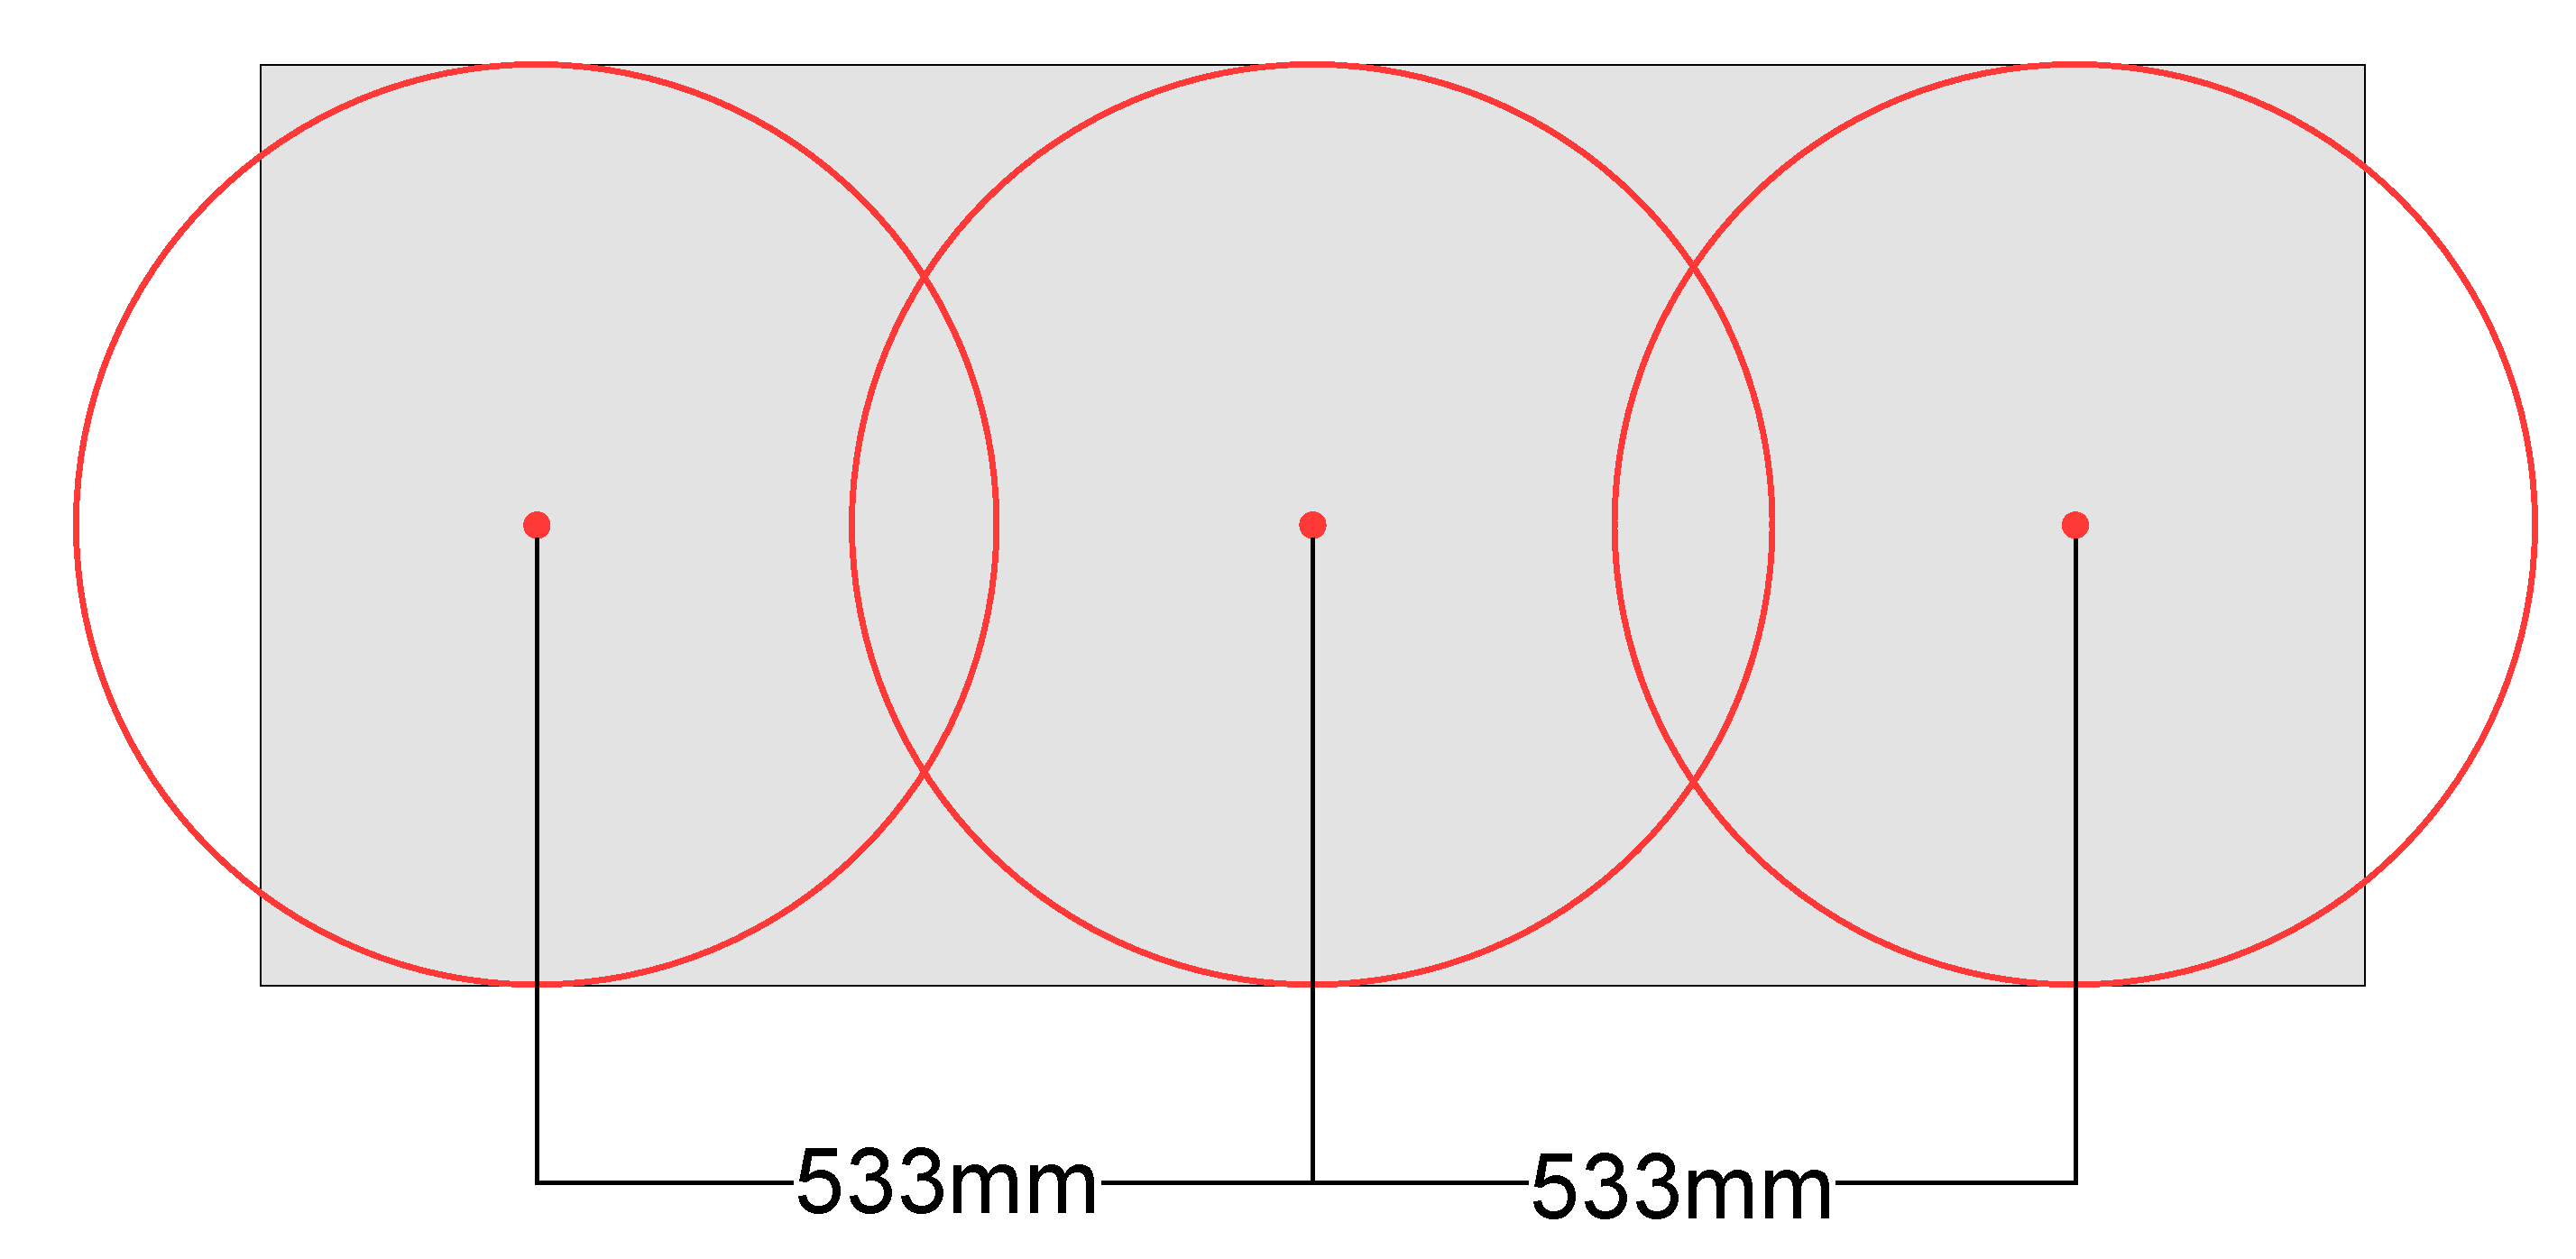
\includegraphics[height=5em]{assets/3transducer.pdf}
    \caption{3个换能器布置方案}
    \label{pic:3个换能器布置方案}
  \end{subfigure}
  \caption{多换能器布置方案}
  \label{pic:多换能器布置方案}
\end{figure}

通过计算,其中方案a(\ref{pic:2个换能器布置方案})的有效振动覆盖率为69\%方案b(\ref{pic:3个换能器布置方案})的有效振动覆盖率为89\%最终确定采用方案b。

\section{结论}

本研究通过试验证明了超声波振动能够降低有机肥施肥机的有机肥与肥箱底板之间的接触阻力,并通过设计正交试验找出了关键影响因素和最佳参数。并且本研究进一步通过有限元仿真确定了最佳的多换能器布置方式。

\end{document}